\label{Introduction}
    In today's world, there are many free and open–source operating systems based on the Linux kernel, called Linux distributions\cite{whatislinux}.  Despite Linux's relatively small market share (between 2.4\% and 4.6\%, to date\cite{linuxmarketshare}), it is being used by millions of people daily and has significant traction among developers\cite{sosurvey} and technically minded people in general.  The companies and communities behind Linux distributions are, of course, trying to raise the usage of their respetive operating systems.  One way to achieve that is through marketing stands at various technical conferences.  Besides persuasion and marketing items such as stickers, a great way to get people to try a new operating system is to simply hand it over to them.

    The community behind the Linux distribution called Fedora\cite{fedora} has been giving out live DVDs which let people try and install Fedora at home.  However, recently a decision was made and Fedora 25 is the last release which will be distributed on DVDs in the European region.  This is because as time advances, less computers actually have a DVD drive.  In the past few years, laptops have been getting thinner and come without DVD drives\cite{laptopdvd}.  Most computers nowadays are capable of booting from an USB flash drive just as well as from disk drives.
    
    The goal of this thesis is to design and construct a device, dubbed the "Fedorator", which will enable writing Fedora to flash drives as a self-service.  The primary use of the Fedorator would be on marketing stands, where it would be available for visitors to use with any USB flash drive.  This device should be relatively simple to construct using off-the-shelf components.
    \section{How Fedora Spreads Publicity}
        The Fedora project has a worldwide Ambassador program.  Ambassadors are people who act as representatives of Fedora.  They have a good understanding of Fedora's principles and aim to spread the message to the public\cite{fedora-ambassadors}.  One of the tasks assigned to Fedora Ambassadors is organizing Fedora participation at events.
        \todo{Discusson over Fedora stands on events and conferences}
        \todo{How DVDs are in use}
        \todo{Ask some people involved in advertisement?}
        \blind[3]
    \section{Rationale for a New Solution}
        Why design and build the Fedorator?  Is there not some existing solution that would prove sufficient?
        
        \subsection{Preloaded USB flash drives}
            Many services offering bulk preloaded USB flash drives may be found on the Internet.  With a large focus on marketing, in general they offer to preload materials such as PowerPoint presentations and PDF prochures\cite{flashbay-data-preloading}.  Literally, they instruct to send the files by email or upload them.  Hence, I'm not sure whether they would be capable of producing bootable USB flash drives.
            
            I went looking to order with the following parameters.
            \begin{itemize}
                \item Capacity of 2GB
                \item 2GB of preloaded data
                \item USB flash drive must be bootable
                \item No branding necessary
                \item 500 units
            \end{itemize}
            
            Most services, rather than showing a cost upfront, ask the user to fill in a form and get a personalized quote.
            
            \todo{ https://www.memorysuppliers.com/ http://www.flashbay.com https://www.premiumusb.com/usb-preloading http://www.memotrek.com/usb/usb-flash-drives-clip-n-easy : 4.19 USD}
        
        \subsection{USB Duplicators}
            Rather than using a service and ordering flash drives already preloaded, we can use dedicated hardware and do the task manually.  There are several products available on the market, called "USB Duplicators", which claim to provide this functionality.  Some examples are provided, with the number of ports and to-date cost in USD and CZK.
            
            \begin{table}[htbp]
            \centering
            \caption{Examples of USB Duplicators}
            \label{usb-duplicators}
                \begin{tabular}{ m{15em}  c  r  r  c }
                \toprule
                    \textbf{Name} & \textbf{ports} & \textbf{USD} & \textbf{CZK} & \\
                \toprule
                Altarec USB Copy Tower SA Duplicator
                 & 118 & \$15~749 & 388~225 CZK & \cite{product-altarec-118} \\
                \hline
                TEAC 1 to 15 USB Drive Duplicator 
                 & 15  & \$1~206  & 29~728 CZK  & \cite{product-teac-15} \\
                \hline
                VINPOWER Black 1 to 11 USBShark USB Flash Copy Tower Duplicator
                 & 11  & \$890    & 21~668 CZK  & \cite{product-vinpower-11}        \\
                \hline
                Altarec USB Copy Cruiser Mini Duplicator\textdagger
                 & 10  & \$315    &  7~764 CZK  & \cite{product-altarec-10}        \\
                \hline
                Intelligent 9 Series (UB910G) - GOLD Factory series 1 - 9 Target USB Flash Memory/Pen Drive/External USB Hard Drive Duplicator
                 & 9   & \$1~260  &  31~056 CZK & \cite{product-intelligent-9}       \\
                \hline
                EZ Dupe 2
                 & 3   & \$81     &   1~997 CZK & \cite{product-ezdupe}       \\
                \hline
                \end{tabular}
            \end{table}
            
            \begin{figure}[htbp]
            \centering
                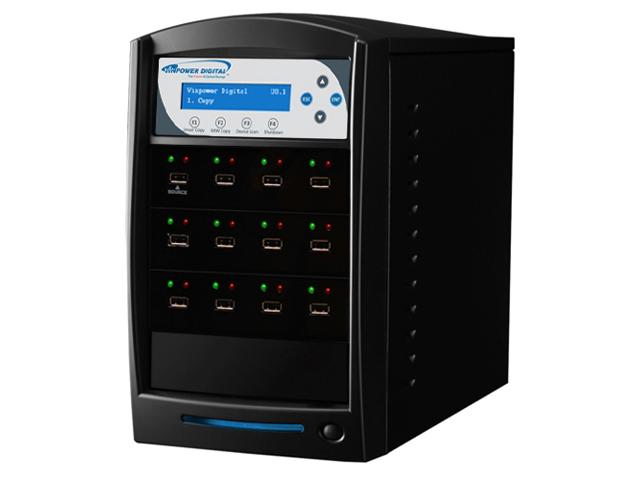
\includegraphics[width=.6\linewidth]{media/vinpower-usbshark.jpg}
                \caption{VINPOWER Black 1 to 11 USBShark \cite{product-vinpower-11}\label{pic:vinpower}}
            \end{figure}
            
            \begin{figure}[htbp]
            \centering
                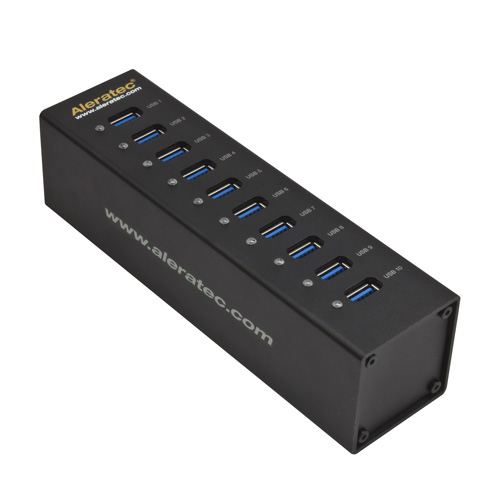
\includegraphics[width=.6\linewidth]{media/altarec-copy-cruiser.jpg}
                \caption{Altarec USB Copy Cruiser Mini Duplicator \cite{product-altarec-10}\label{pic:altarec}}
            \end{figure}
            
            In general, the products can be split into two categories: devices that work stand-alone and devices that require a computer to operate.  Devices from the latter category were marked with a dagger (\textdagger).
            
            Besides their price, the trouble with these products is that they are proprietary.  The hardware cannot be built from scratch and the software cannot be inspected or improved.  The devices which are not stand-alone require a computer with specific software and drivers to operate.  Linux support is not claimed, and therefore likely unavailable, leading to a sad and undesired irony of requiring a computer running an OS that is not Linux in order to produce and distribute USB flash drives containing Linux.
        \subsection{}
            \todo{Doing it by hand?}
